%\svnidlong
%{$HeadURL$}
%{$LastChangedDate$}
%{$LastChangedRevision$}
%{$LastChangedBy$}
%\svnid{$Id: $}


%%%%%%%%%%%%%%%%%%%%%%%%%%%%%%%%%%%%%%%%%%%%
%\section*{EFT Validity and Truncation Summary}
%%%%%%%%%%%%%%%%%%%%%%%%%%%%%%%%%%%%%%%%%%%%

Most of this report has focused on simplified models of dark matter.
In this Chapter, we wish to emphasize the applicability of
Effective Field Theories (EFTs) 
in the interpretation of DM searches at the LHC.
Given our current lack of knowledge about the nature of a DM particle and
its interactions, it appears mandatory to provide the necessary information
for a model independent interpretation of the collider bounds.
This approach should be complemented with
an interpretation within a choice of simplified models.
We note that, even though EFT benchmarks are only valid in given conditions,
the results provided by the current list of simplified models cannot always
characterize the breadth of SM-DM interactions.
In at least one case, composite WIMPs~\cite{Nussinov:1985xr,Kaplan:1991ah,Banks:2010eh}, 
the contact interaction framework is the correct one to
constrain new confinement scales. 

Ideally, experimental constraints should be shown as bounds of allowed signal events in the kinematic regions considered for 
the search, as detailed in Appendix~\ref{app:Presentation_Of_Experimental_Results}. 
A problematic situation is the attempt to derive a limit on
nucleon-dark matter scattering cross sections from EFT results
based on collider data~\footnote{Comparisons between constraints from different experiments 
	meant to highlight their complementarity should be expressed as 
	a function of the model parameters rather than on derived observables;
	however this is a point that should be developed further after the conclusion of the work of this Forum.}. 
Experiments that directly probe the nucleon-dark matter scattering cross section 
are testing the regime of small momentum transfers, where the EFT approximation typically holds.  
Collider experiments, though, are sensitive to large momentum transfers: 
We first illustrate the complications
that can arise with EFTs at colliders by considering an effective interaction
$$ {\cal L}_\textrm{int} = {(\bar q\gamma_\mu q)(\bar\chiDM\gamma^\mu\chiDM) \over \Mstar^2}
= (\bar q\gamma_\mu q)(\bar\chiDM\gamma^\mu\chiDM) {g\over \Lambda^2}$$
that couples quarks and DM $\chi$ fields.\footnote{The \textit{exact} operator chosen is not important:
	as detailed in the following, statements concerning the applicability of an EFT can also be made without a specific relation to simplified models.}  
The strength of this interaction is
parametrized by $\displaystyle {1\over \Mstar^2} = {g\over \Lambda^2}$.
A monojet signature can be generated from this operator
by applying perturbation theory in the QCD coupling.
An experimental search will place a limit on \Mstar.   
For a fixed \Mstar, a small value of $g$ will correspond
to a small value of $\Lambda$.   The EFT approximation breaks down
if $Q>\Lambda$, where $Q$ is a typical hard scale of the process.
The limit on small $g$ can only be reliable if the
kinematic region $Q>\Lambda$ is removed from the event generation.
However, if a fraction of events is removed from the prediction,
the corresponding value of $g$ must increase to match the experimental
limit on \Mstar.
On the other hand, if, for the same value of \Mstar, a large $\Lambda$
is assumed so that the full set of events fulfill the EFT validity condition,
a larger value of $g$ is required.  For large enough $g$, computations based on perturbation theory become unreliable.

In the first part of this Chapter, we summarize two methods that
have been advocated to truncate events that 
do not fulfill the condition necessary for the use of an EFT.
These methods are described in detail in Refs.~\cite{Busoni:2013lha,Busoni:2014sya,Busoni:2014haa,Aad:2015zva,Racco:2015dxa,Berlin:2014cfa}. 
We then propose a recommendation for the presentation of EFT results for early Run-2 LHC searches.

\section{Procedures for the truncation of EFT benchmark models}

%%%%%%%%%%%%%%%%%%%%%%%%%%%%%%%%%%%%%%%%%%%%
\subsection{EFT truncation using the momentum transfer and information on UV completion}

\label{sec:TruncationWithQTr}
%%%%%%%%%%%%%%%%%%%%%%%%%%%%%%%%%%%%%%%%%%%%

In the approach described in Ref.~\cite{Busoni:2014sya},
the EFT prediction is modified to incorporate the effect of a
propagator for a relatively light mediator.
For a tree-level interaction between DM and
the SM via some mediator with mass \mMed, 
the EFT approximation corresponds to expanding the propagator
for the mediator
in powers of $\Qtr^2/\mMed^2$, truncating at lowest order, and combining the remaining parameters into a single parameter \Mstar 
(connected to the scale of the interaction $\Lambda$ in the literature).
For an example scenario with a \Zprime-type mediator (leading to some combination of operators D5 to D8 in the notation of~\cite{Goodman:2010ku} for the EFT limit),
this corresponds to setting
\be
\frac{\gDM \gq}{Q_{\rm tr}^2-\mMed^2}=-\frac{\gDM \gq}{\mMed^2}\left(1+\frac{Q^2_{\rm tr}}{\mMed^2}+ \mathcal{O} \left(\frac{Q^4_{\rm tr}}{\mMed^4}\right)\right) \simeq -\frac{1}{{\Mstar^2}},
\ee
%
where $\Qtr$ is the momentum carried by the mediator, and $\gDM$,
$\gq$ are the DM-mediator and quark-mediator couplings
respectively.\footnote{Here, we ignore potential complications from
the mediator width when the couplings are large.}
A minimal condition that must be satisfied for this approximation to be valid is that $\Qtr^2 < \mMed^2 = \gDM \gq {\Mstar^2}$.
This requirement avoids the regions:
$\Qtr^2 \sim \mMed^2$, in which case the EFT misses a resonant enhancement, and it is conservative to ignore this enhancement;
and $\Qtr^2 \gg \mMed^2$, in which case the signal cross section
should fall according to a power of $\Qtr^{-1}$ instead of $\mMed^{-1}$.   The latter is the problematic kinematic region.

The condition $\Qtr^2 < \mMed^2 = \gDM \gq \Mstar^2$ was applied
to restrict the
kinematics of the signal and remove events for which the high-mediator-mass approximation made in the EFT would not be reliable.
This leads to a smaller effective cross-section, after imposing the event selection of the analysis.  This truncated signal was then used
to derive a new, more conservative limit on
$\Mstar$ as a function of $(\mDM, \gDM \gq)$.

For the example D5-like operator,
where the cross section $\sigma$ scales as $\Mstar^{-4}$,
there is a simple rule for converting a rescaled cross section into a rescaled constraint on ${\Mstar}$.
if the original limit is based on a simple cut-and-count procedure.
%CD: I would keep it
Defining $\sigma_{\rm EFT}^{\rm cut}$ as the cross section truncated such that all events pass the condition $\sqrt{\gDM \gq} \Mstar^{\rm rescaled} > \Qtr$, we have
\be
\Mstar^{\rm rescaled} = \left(\frac{\sigma_{\rm EFT}}{\sigma_{\rm EFT}^{\rm cut}(\Mstar^{\rm rescaled})}\right)^{1/4} \Mstar^{\rm original},
\ee
%
which can be solved for $\Mstar^{\rm rescaled}$ via either iteration or a scan.
Similar relations exist for a given UV completion of each operator. 

This procedure has been proposed in Ref.~\cite{Busoni:2014sya} 
and its application to ATLAS results can
be found in Ref.~\cite{Aad:2015zva} for a range of operators.
We reiterate: knowledge of the UV completion for a given
EFT operator was necessary for this procedure;
this introduces a model-dependence that was not present
in the non-truncated EFT results. 

Currently, simplified models (including the full effect
of the mediator propagator) are available for comparison with
the data, and since knowledge of the simplified models is needed
for the truncation procedure,
there is no reason to apply this prescription.   Instead, the
simplified model limit for large \Mstar can be presented for
interpretation in terms of EFT operators.


%%%%%%%%%%%%%%%%%%%%%%%%%%%%%%%%%%%%%%%%%%%%
\subsection{EFT truncation using the center of mass energy}
\label{sec:TruncationWithSHat}
%%%%%%%%%%%%%%%%%%%%%%%%%%%%%%%%%%%%%%%%%%%%

The procedure presented in the previous section was predicated on
some knowledge of the simplified model.  This led to the identification
of the mass of the DM pair as the relevant kinematic quantity to use
in a truncation procedure.
In general, if no assumption is made about the underlying dynamics,
it is more conservative to place a limit on the total center
of mass energy $E_\text{cm}$ of the DM production process.
Furthermore, the direct connection between the mass scale of
the EFT validity, \Mcut, and the
mass scale that normalizes the EFT operator, \Mstar, is unknown.
For such cases,~Refs.\cite{Racco:2015dxa,Berlin:2014cfa} proposed
a procedure to extract model independent and consistent bounds within the EFT
that can be applied to any effective Lagrangian describing the interactions between the DM and the SM.
This procedure provides conservative limits that can be directly reinterpreted in any completion of the EFT.
The condition ensuring that the EFT approximation is appropriate is:
\begin{equation}
\label{Ecm<Mcut}
E_\text{cm}<M_\text{cut}\,.
\end{equation}

The relationship between \Mcut and \Mstar can be parameterized
by an \textit{effective coupling strength} \gstar, such that
$\Mcut=\gstar \, \Mstar\,.$
A scan over values of \gstar provides an indication of the
sensitivity of the prediction to the truncation procedure.
In the \Zprime-type model considered above, \gstar is equal to $\sqrt{\gDM\gq}$.
%
The resulting plots are shown in \cite{Racco:2015dxa} for a particular effective operator. 

The advantage of this procedure is that the obtained bounds can be directly and easily recast in any  completion of the EFT, by computing the parameters \Mstar, \Mcut in the full model as functions of the parameters of the complete theory. On the other hand, the resulting limits will be weaker than those obtained using \Qtr and a specific UV completion.

\subsection{Truncation at the generator level}

The conditions on the momentum transfer can also be applied directly at the generator level, by discarding 
events that are invalid and calculating the limits from this truncated shape. 
This provides the necessary rescaling of the cross section while keeping the information on the change in the kinematic distributions due to the removal of the invalid events. This procedure is more general with 
respect to rescaling the limit in the two sections above, and it should be followed if
a search is not simply a counting experiment and exploits the shapes of kinematic distributions.

\subsection{Sample results of EFT truncation procedures}

An example of the application of the two procedures to the limit on \Mstar from Ref.~\cite{ATL-PHYS-PUB-2014-007} as a function of the product of the couplings is shown in Figure~\ref{Ecm<Mcut}. Only the region between the dashed and the solid line is excluded. It can be seen that the procedure from~\cite{Racco:2015dxa} outlined in Section~\ref{sec:TruncationWithSHat}, shown in blue, is more conservative than the procedure from Refs.~\cite{Busoni:2014sya,Aad:2015zva}, described in Section~\ref{sec:TruncationWithQTr}.

\begin{figure}
	\centering
	\includegraphics[width=0.95\textwidth]{figures/EFT/MstarLimitvscouplingSec600_Stop13_R0_DM_EFT_D5_DM50_tree.pdf}
	\caption{95\% CL lower limits on the scale of the interaction of the D5 operator at 14~\tev, after the two truncation procedures. 
		The procedure from~\cite{Racco:2015dxa} outlined in Section~\ref{sec:TruncationWithSHat} is shown in blue, while the procedure from Refs.~\cite{Busoni:2014sya,Aad:2015zva}, described in Section~\ref{sec:TruncationWithQTr} is shown in red. Only the region between the dashed and the solid lines is excluded. Even though the intersection between the two lines is not shown in this plot, it should be noted that no limit can be set anymore for sufficiently low couplings, whatever truncation method is used.}
	\label{fig:monojet_MstarMmed}
\end{figure}


\subsection{Comments on unitarity considerations}

A further consideration applicable to EFT operators at hadron colliders
is the potential violation of unitarity.  An analysis of the operator
$\displaystyle {\bar{q}\gamma_\mu q\bar\chi\gamma^\mu\chi \over \Mstar^2}$
provides the limit:
\be
\Mstar > \beta(s) \sqrt{s}  \sqrt{ {\sqrt{3} \over 4 \pi}  },
\ee
where $\sqrt{s}$ is (maximally) the collider energy and $\beta(s)$ is
the DM velocity \cite{Shoemaker:2011vi}.
Constraints for other operators have also been derived \cite{Endo:2014mja}.
This constraint on \Mstar still is open to interpretation, since the
relation to \Mcut is not resolved, except for a specific simplified model.
Derived limits on \Mstar should be compared to this unitarity bound to
check for consistency.


\section{Recommendation for presentation of EFT results} %change this title
\label{sec:RecommendationEFTResults}

In this report,
we make two recommendations for the presentation of collider results
in terms of Effective Field Theories for the upcoming Run-2 searches. 
A full discussion of the presentation of
collider results in relation to other experiments
is left to work beyond this Forum, where ATLAS, CMS, the theory community
and the Direct and Indirect Detection communities are to be involved. 

We divide the EFT operators in two categories: 
those that can be mapped to one or more UV-complete simplified models, such as those
commonly used in LHC searches so far and detailed in~\cite{Goodman:2010ku}, and those
for which no UV completion is available to LHC experiments, such as those outlined in Section~\ref{sec:EFT_models_with_direct_DM_boson_couplings}.

\subsection{EFT benchmarks with corresponding simplified models}
\label{sub:EFT_withSimp}

If a simplified model can be mapped to a given EFT, then the model's high-mediator-mass limit  will converge to the EFT.
A study of 14 TeV benchmarks for narrow resonances with \gq = 0.25 and \gDM = 1 (see Section~\ref{sub:parameter_scan_monojet})
shows that a mediator with a mass of at least 10 TeV fully reproduces the kinematics of a contact
interaction and has no remaining dependence on the presence of a resonance. 
A comparison of the main kinematic variables for the \schannel vector 
mediator model with a width of 0.1 \mMed
is shown in Fig.~\ref{fig:EFT_kinematics}.\footnote{The use of a fixed width rather than the minimal width is exclusive of these plots.} 

\begin{figure*}[p!]
	\centering
	\subfloat[\MET{}]{
		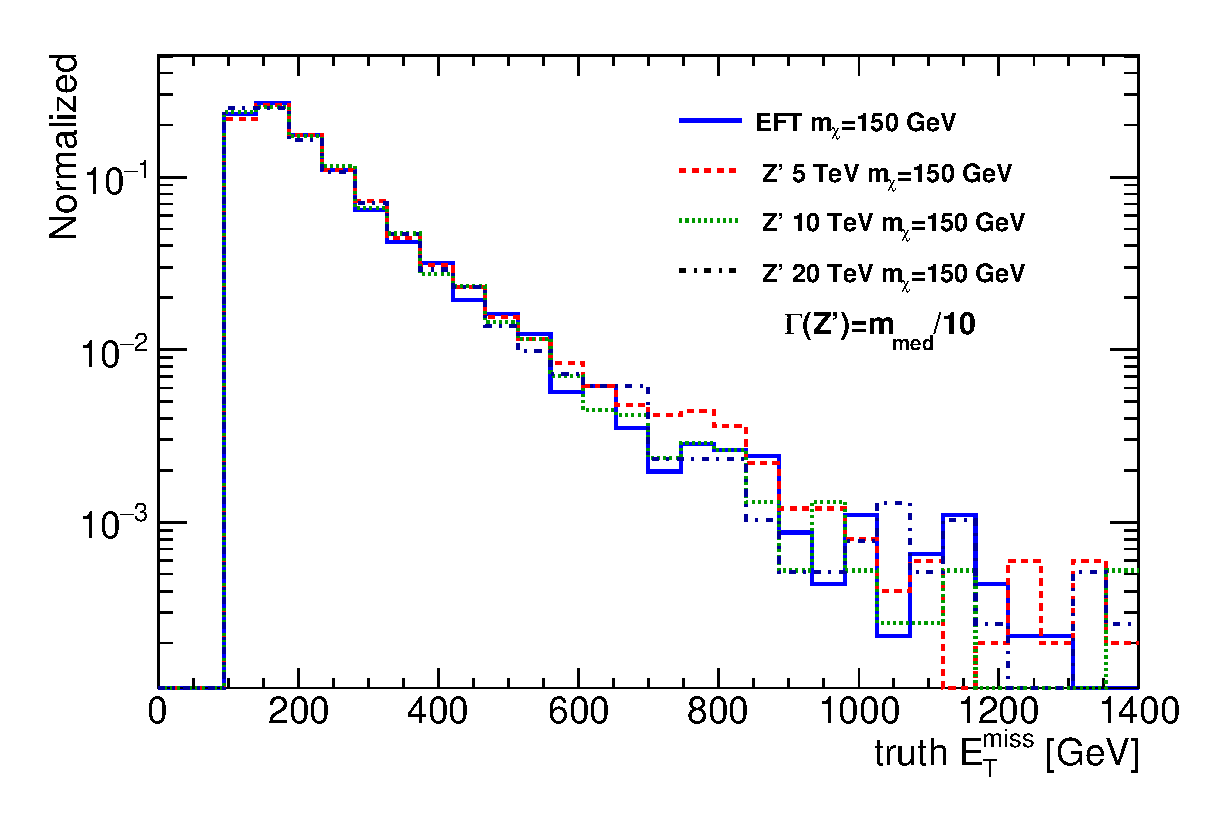
\includegraphics[width=0.5\linewidth]{figures/EFT/TruthETmiss_compEFTvsZprime_DM150_narrow}
	}
		\hfill
	\subfloat[Center of mass energy $E_{cm}$]{
	   \includegraphics[width=0.47\linewidth]{figures/EFT/TruthEcm_compEFTvsZprime_DM150_narrow} 
	}		
	\subfloat[Mediator transverse momentum]{
		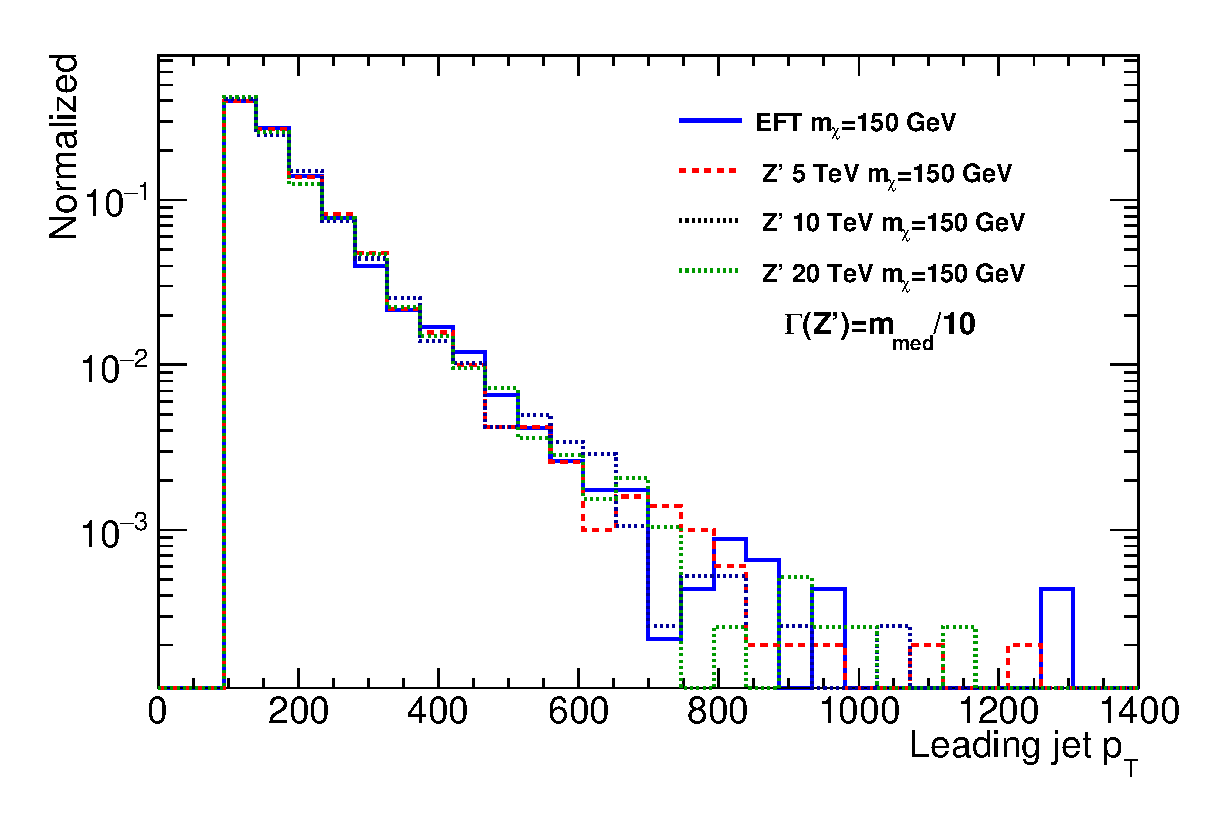
\includegraphics[width=0.47\linewidth]{figures/EFT/TruthPt_compEFTvsZprime_DM150_narrow}
	}
		\hfill
	\subfloat[Leading DM transverse momentum]{
		\includegraphics[width=0.47\linewidth]{figures/EFT/TruthDM1ptcompEFTvsZprime_DM150_narrow} 
		}
	\subfloat[DM transverse momentum (sub-leading)]{
		\includegraphics[width=0.47\linewidth]{figures/EFT/TruthDM2ptcompEFTvsZprime_DM150_narrow} 
	}
	\vskip20pt
		\caption{Comparison of the kinematic distributions at 14~\tev between a narrow \schannel mediator and the
			corresponding D5 contact operator, at generator level for a jet+\MET{} signature. 
			\label{fig:EFT_kinematics}}
		
\end{figure*}



As already observed in Section~\ref{sub:parameter_scan_monojet}, varying the DM mass changes the kinematics,
both in the simplified model and in the EFT case. This can be seen in Fig.~\ref{fig:EFT_kinematics_mDM}. 

\begin{figure*}[p!]
	\centering
	\subfloat[\MET{}, D5 operator]{
		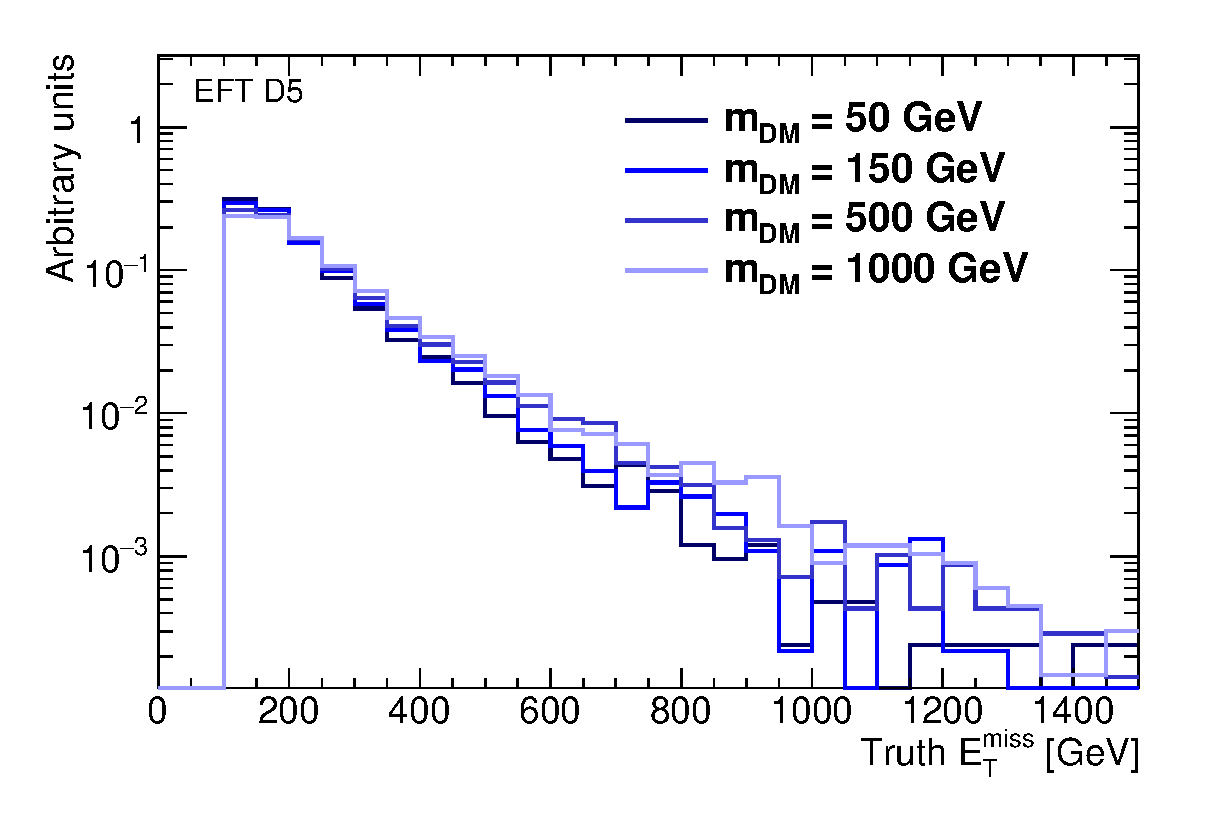
\includegraphics[width=0.47\linewidth]{figures/EFT/EFT_met}
	}
	\subfloat[Invariant mass of the two WIMPs $m_{\chi \chi}$, D5 operator]{
		\includegraphics[width=0.47\linewidth]{figures/EFT/EFT_shat} 
	}		
	\hfill
	\subfloat[\MET{}, simplified model]{
		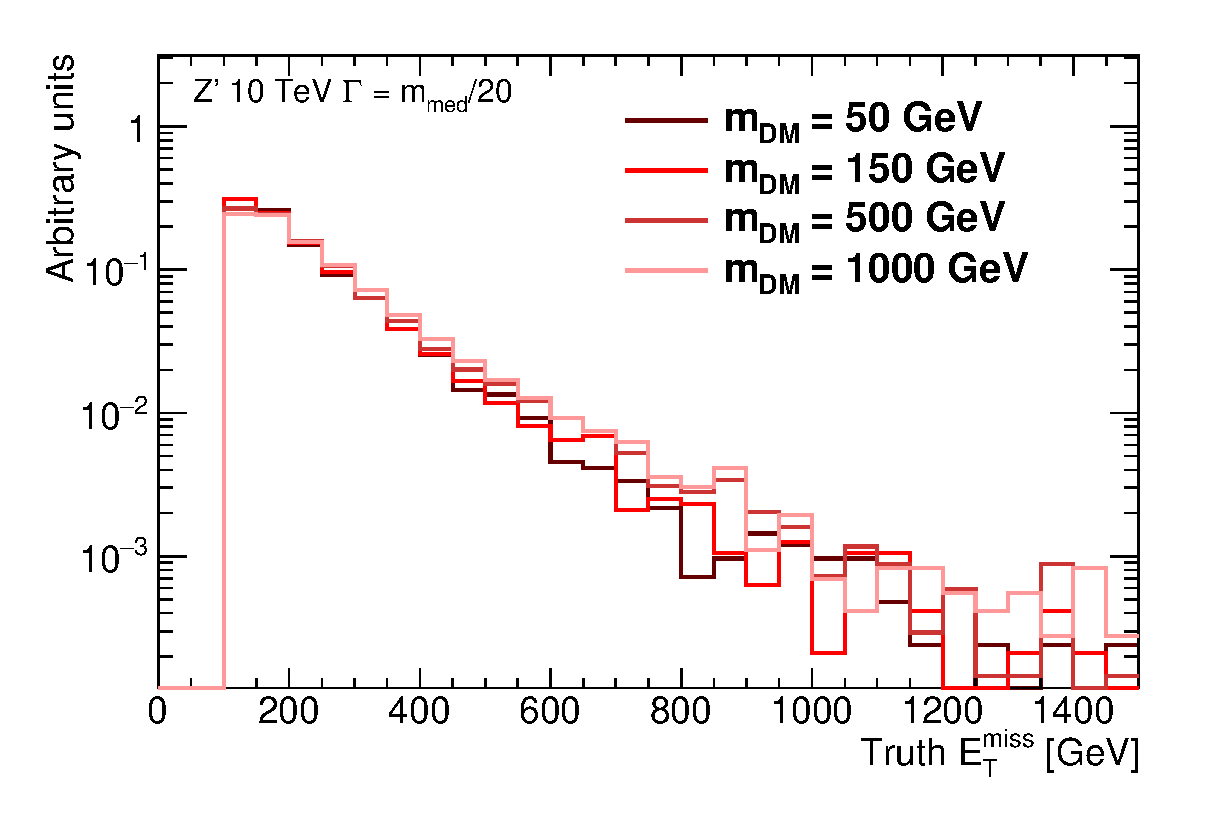
\includegraphics[width=0.47\linewidth]{figures/EFT/Zprime_met}
	}
	\subfloat[Invariant mass of the two WIMPs $m_{\chi \chi}$, simplified model]{
		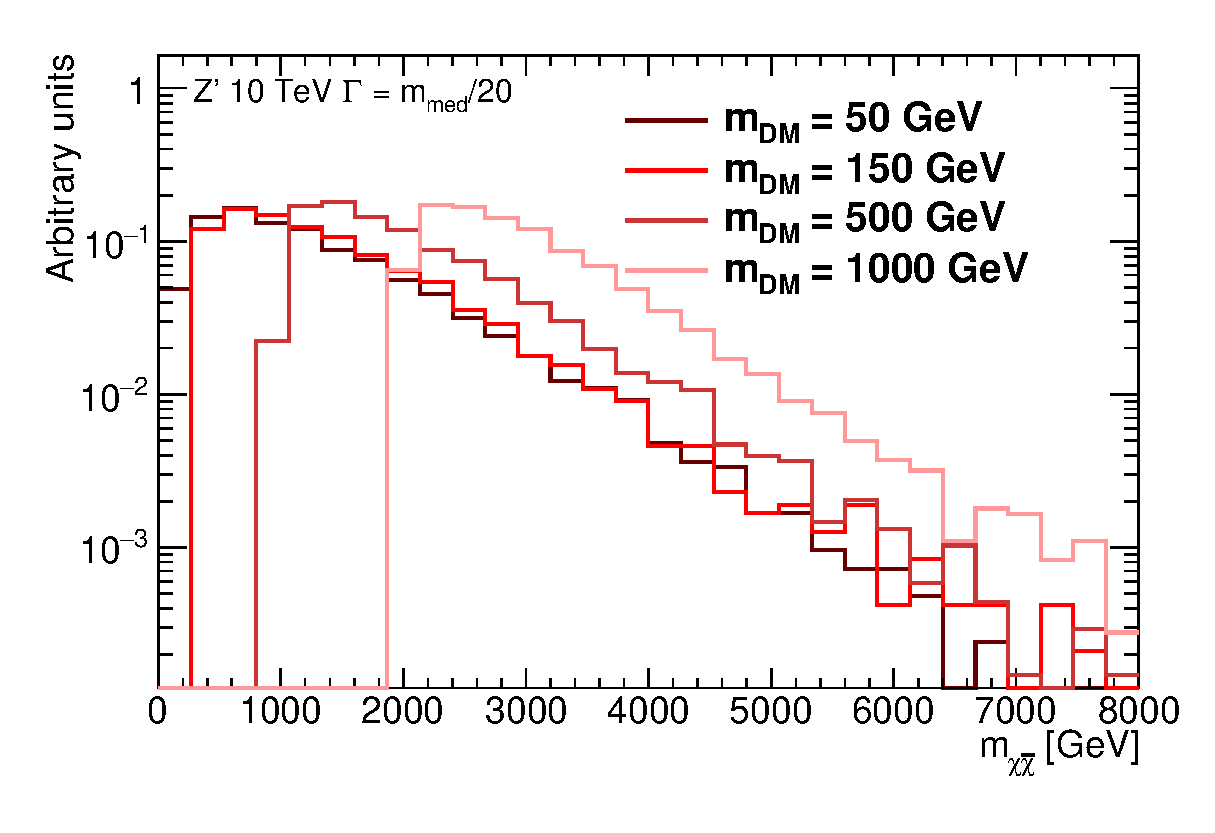
\includegraphics[width=0.47\linewidth]{figures/EFT/Zprime_shat} 
	}		
	\caption[][28pt]{Comparison of the kinematic distributions for a narrow \schannel mediator, 
		at generator level for a jet+\MET{} signature, for varying DM masses. 
		\label{fig:EFT_kinematics_mDM}}
\end{figure*}

\vskip20pt
	
Based on these studies, the Forum recommends experimental collaborations to 
add one grid scan point at very high mediator mass (10 \tev) to the scan, 
for each of the DM masses for the \schannel simplified models described in Section~\ref{subsec:MonojetLikeModels}. 
This will allow to reproduce the results of an equivalent contact interaction
as a simple extension of the existing parameter scan. 

It should be checked that the high-mass mediator case for the simplified model is correctly implemented 

%% (3) truncate using \Ecm.  The reliability of the EFT approximation can

Whenever a UV completion is not available, an EFT still
captures a range of possible theories beyond the simplified models that we already consider. 
However, in the case of the dimension-7 operators detailed in Section~\ref{sec:EFT_models_with_direct_DM_boson_couplings}
we can only roughly control how well the EFT approximation holds, as described in Section~\ref{sub:validityEWContact}.
Despite the fact that a propagator was introduced to motivate
the truncation procedure for \schannel models, the prescription from Sec.~\ref{sub:EFT_withSimp}
depends upon the simplified model to derive the
energy scaling that is used for the comparison with the momentum transfer. 
The simple fact remains that the effective
coupling of the operator -- $g/\Lambda^n$ -- should not allow
momentum flow $Q>\Lambda$ or $g>4\pi$.  Given our ignorance of
the actual kinematics, 
the truncation procedure recommended for this purpose
is the one described in Section~\ref{sec:TruncationWithSHat},
as it is independent from any UV completion details. 

Because there is no UV completion,
the parameter \Mcut can be treated more freely than
an explicit function of $g$ and $\Lambda$.
It makes sense to choose \Mcut such that we 
identify the transition region where the EFT stops being
a good description of UV complete 
theories. This can be done using the ratio \Reft, which is defined
as the fraction of events for which $\hat{s} > \Mcut^2$. 
For large values of \Mcut, no events are thrown away in the truncation 
procedure, and \Reft = 1. As \Mcut becomes smaller, eventually all events are thrown 
away in the truncation procedure, i.e. \Reft = 0, and the EFT gives no 
exclusion limits for the chosen acceptance.  

We propose a rough scan over \Mcut, such that we find the values of \Mcut 
for which \Reft ranges from 0.1 to 1. The analysis can then perform a scan over 
several values of \Mcut, and show the truncated limit 
for each one of them. 
